\section{Cholesky Decomposition}

The Cholesky decomposition is a mathematical procedure that enables to speed up many applications in theoretical chemistry. It allows to decompose a hermitian, positive (semi-)definite matrix $M$ into a lower triangular matrix $L$ and its transposed

\begin{equation}
M=LL^T.
\end{equation}

It can for example be applied to decompose the two-electron four-center integral matrix  into three index objects

\begin{equation}\label{CDMatrix}
\langle \mu \nu | \lambda \sigma \rangle = \sum_P^M \langle \mu \nu | P \rangle \langle P | \lambda \sigma \rangle = \sum_P^M L^P_{\mu\nu} L^P_{\lambda\sigma} ,
\end{equation}

where the greek letters are indices of the basis functions $\phi_\mu$ and the counting index $P$ refers to which Cholesky vector is used. This Cholesky vector is equivalent to the $P$th column in the matrix $L$. Consequently, $M$ is the number of Columns in $L$ or the number of Cholesky vectors. The mapping of the column or row indices of the original matrix to the indices of the Choleky vectors is called the Cholesky basis.\\

To see why this decomposition is useful in speeding up calculations, one can compare it to the well established resolution of the identity (RI) approach. Here, the basis is projected to the space of a prefitted auxiliary basis so that it seems that the identity of the auxiliary basis was inserted into the original expression
\begin{equation}\label{RIFull}
\langle \mu \nu | \lambda \sigma \rangle \approx \sum_{P,Q} \langle \mu \nu | P \rangle \langle P | Q \rangle^{-1} \langle Q | \lambda \sigma \rangle .
\end{equation} 

If simplified using

\begin{equation}
B_{\mu \nu,Q} = \sum_{P} \langle \mu \nu | P \rangle \langle P | Q \rangle^{-1/2},
\end{equation}

the equation becomes 

\begin{equation}
\langle \mu \nu | \lambda \sigma \rangle \approx \sum_{Q} B_{\mu \nu,Q} B_{\lambda \sigma,Q}.
\end{equation} 

Comparing this result to Eq.~\ref{CDMatrix} it becomes evident that they are equivalent and can be evaluated with similar efficiency. However, one has to keep in mind that, in general, the basis obtained in all Cholesky procedures is larger than the prefitted auxiliary basis sets used in the RI approach. As a result, Cholesky based calculations will always be slower than comparable RI calculations if available.\\

The advantage of Cholesky Decomposition compared to RI is that, as shown in the following sections, it offers error control for all elements in the matrix that is decomposed. This is in contrast to the RI approach, where the auxiliary basis is fitted to reproduce on particular metric (like for example the Coulomb energy contribution), but a reconstruction of the original matrix as in Eq.~\ref{RIFull} will contain significant errors.


\subsection{The Decomposition Algorithm}

A basic algorithm to perform the Cholesky decomposition is given below (Algorithm 1). It features pivoting, which means that no full decomposition is performed but that the decomposition is stopped once a certain accuracy in each matrix element (given by the decomposition threshold $\delta$ ) is reached. The drawback of this algorithm is that it requires the original matrix $M$ to be stored in memory in its entirety. This normally is no problem but the full two-electron four-center integrals can quickly take up more memory than available in modern clusters.

\begin{figure}[h!]
	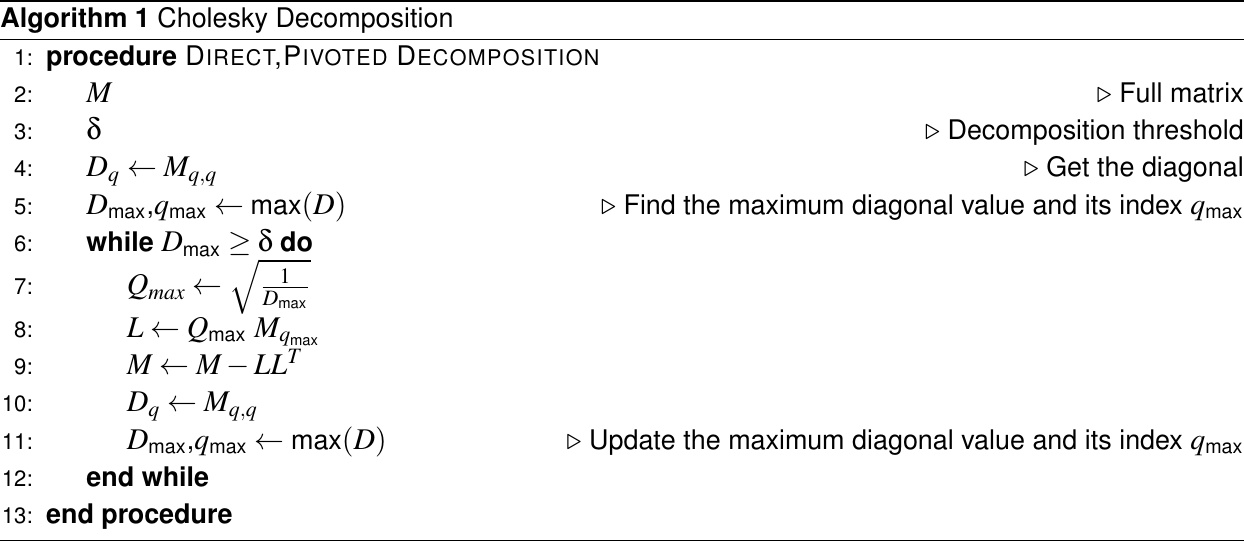
\includegraphics[width=\textwidth]{cholesky/algorithm1.png}
\end{figure}

To circumvent this problem, a memory efficient algorithm is implemented in \textsc{Serenity} (Algorithm 2). This algorithm firstly analyzes the diagonal to find the columns that have the potential to contribute to the Cholesky vectors and summarizes the corresponding indices in the reduced set $\mathcal{R}$. Then, the most significant elements in $\mathcal{R}$ are determined and summarized in the qualified set $\mathcal{Q}$. In general, this set is obtained by checking if the diagonal element is larger than $D_\text{min}$ but, in practice, the size of $\mathcal{Q}$ is also limited to a smaller number of elements to ensure memory and general efficiency (this avoids the calculation and later subtraction of too many elements that ultimately do not contribute to the Cholesky vectors, due to linear dependencies in $\mathcal{Q}$). As a result, in each iteration only the subset of integrals spanned by $\mathcal{Q}$ and $\mathcal{R}$ has to be calculated. Furthermore, the quite expensive subtraction step only has to be performed on that subset of integrals during each iteration. This also means that, in the end, the Choleksy vectors are calculated only in the subspace of $\mathcal{R}$ and have to be mapped to the corresponding indices in the complete set $\mathcal{S}$. Another important feature of this algorithm is checking for numerical errors. These can lead to small negative entries in the diagonal, which in turn can lead to errors in the calculation of $Q_{\text{max}}$. The last feature worth mentioning is the pre-screening of the qualified set $\mathcal{Q}$ for all elements that will actually contribute to the Cholesky vectors. This step exploits the fact that a decomposition of a matrix spanned by $\mathcal{Q}$ and $\mathcal{R}$ will yield the same contributing indices as the decomposition of the matrix spanned by $\mathcal{Q}$ and $\mathcal{Q}$. Since the dimension of $\mathcal{Q}$ is significantly lower than that of $\mathcal{R}$, the overhead created by additional decomposition step is negligible compared to the computational savings in the following steps.

\begin{figure}
	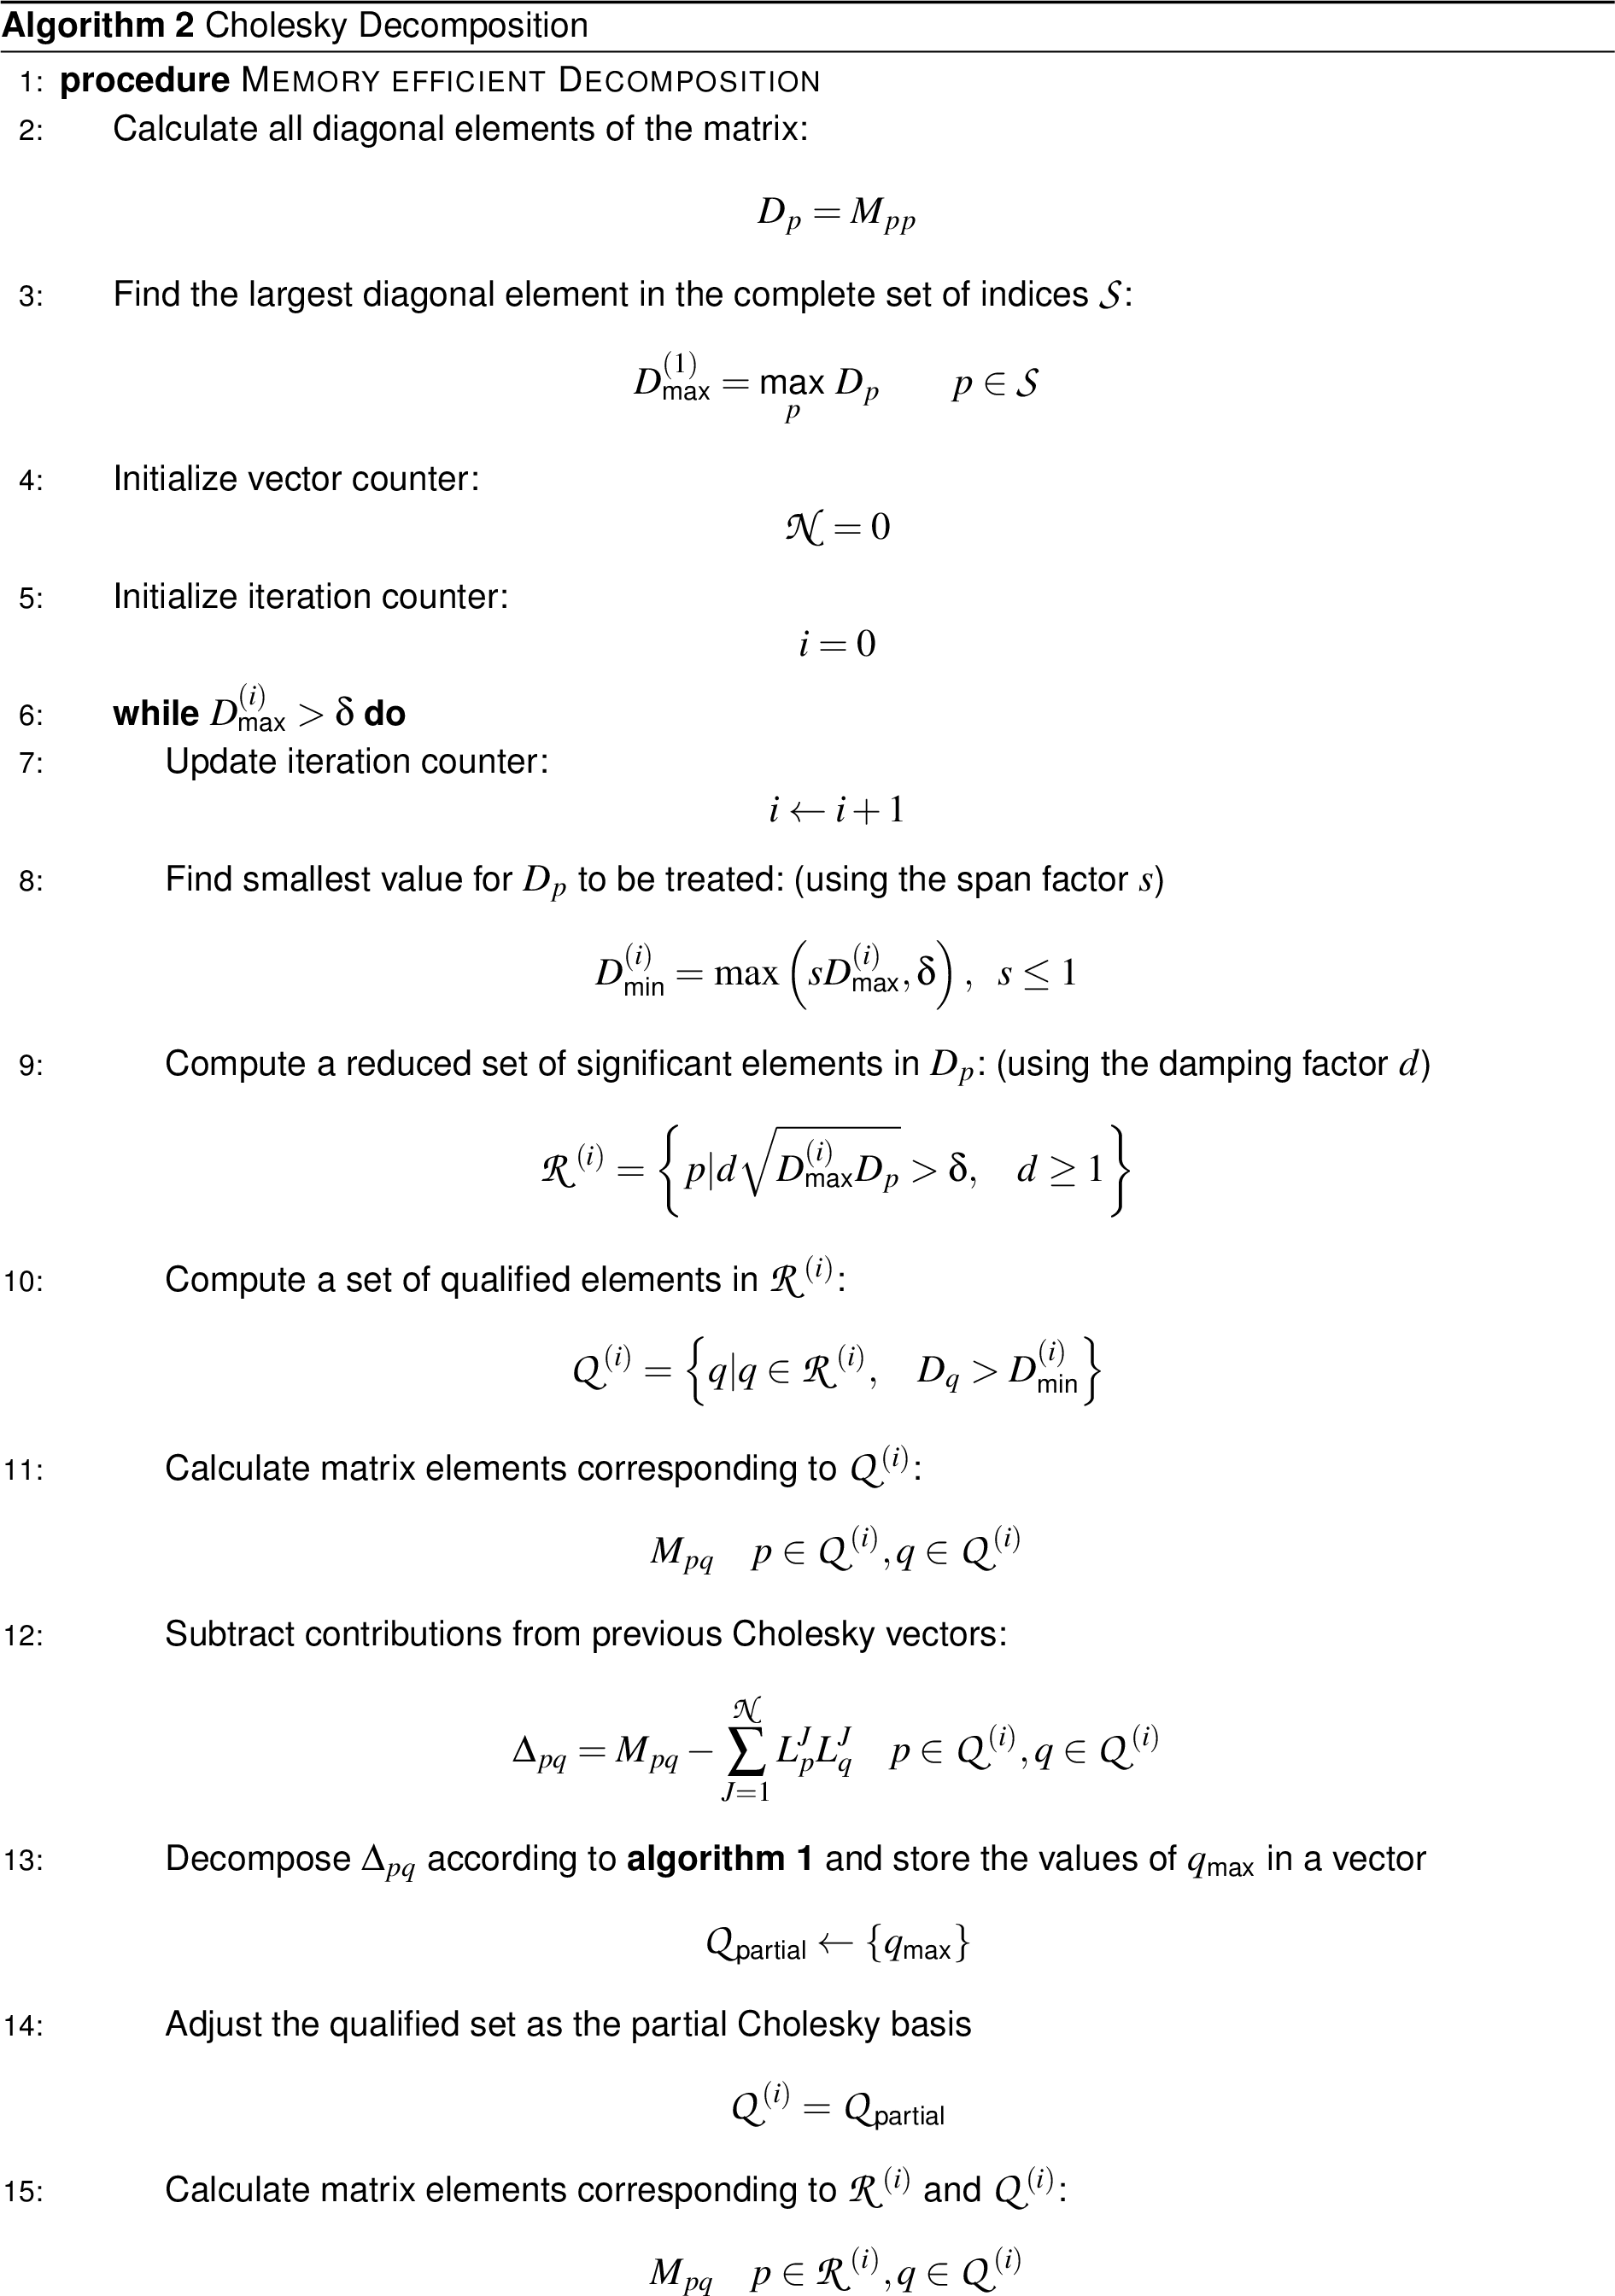
\includegraphics[width=\textwidth]{cholesky/algorithm2_1.png}
\end{figure}

\begin{figure}
	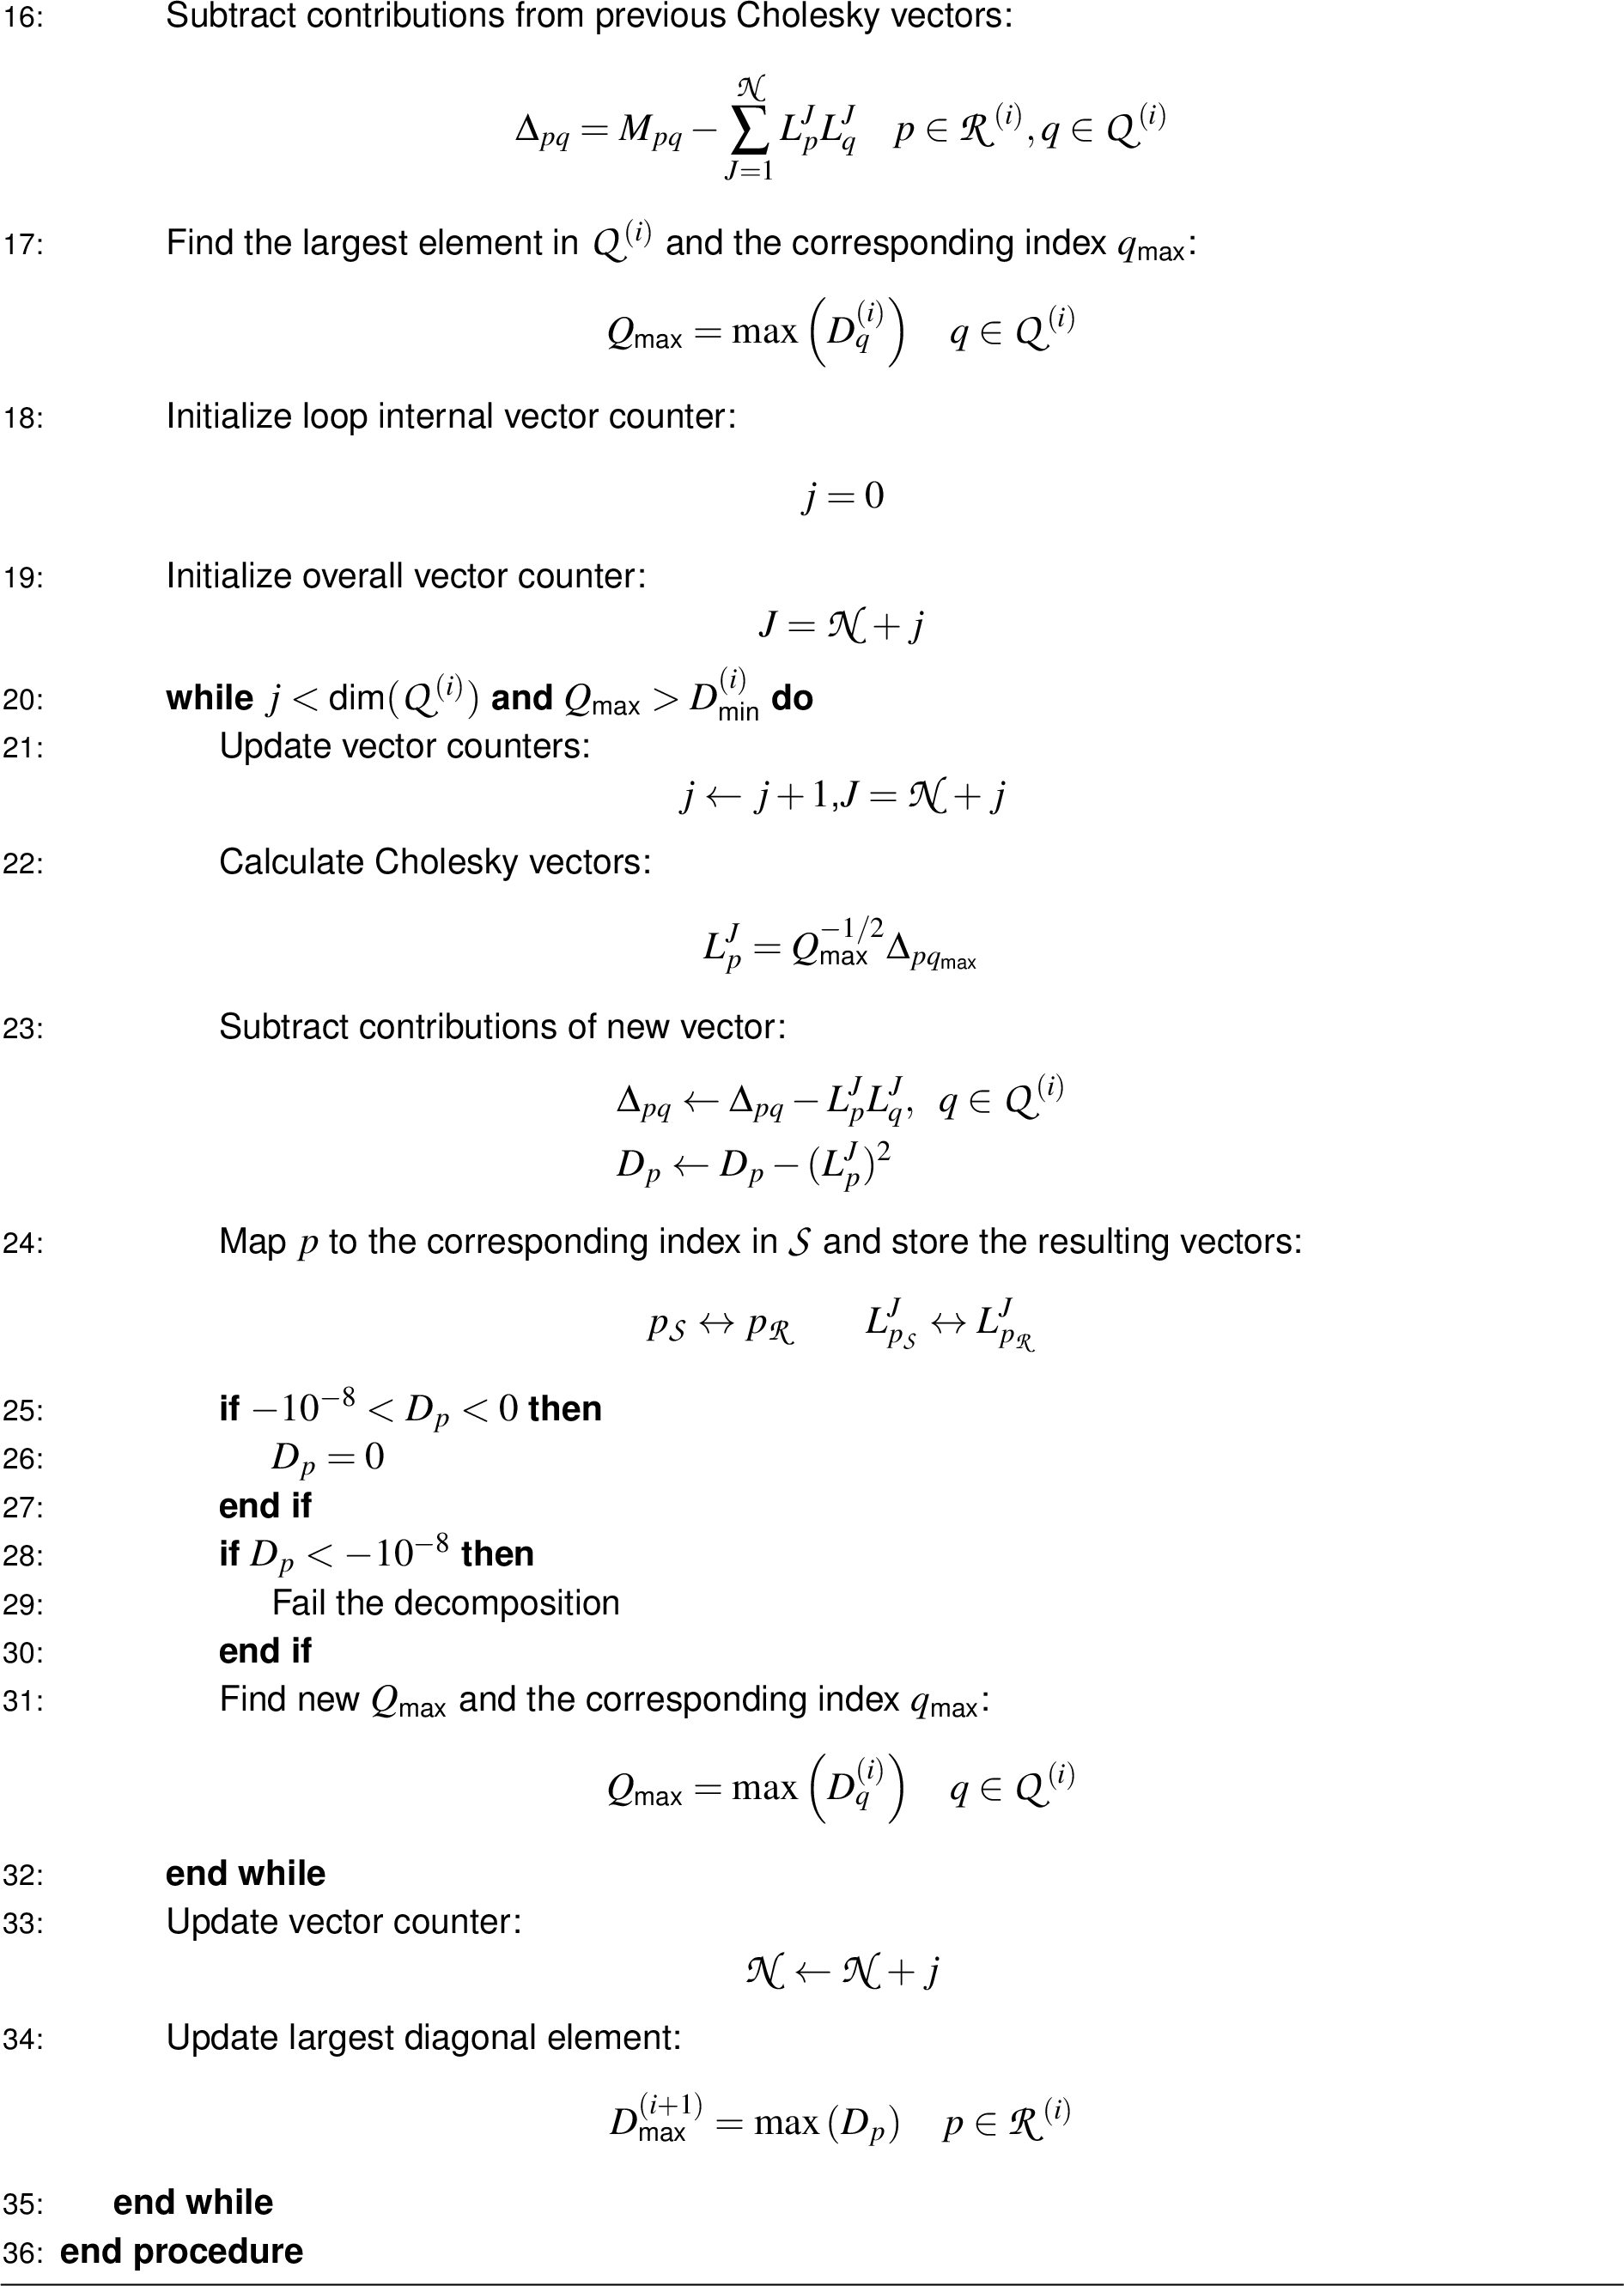
\includegraphics[width=\textwidth]{cholesky/algorithm2_2.png}
\end{figure}



\subsection{The Atomic Cholesky Decomposition}

One major problem of the generic Cholesky decomposition approach is that it needs to decompose the complete two-electron four-center integral matrix. This is easily feasible for small systems, but at the latest when it is no longer possible to hold the full matrix in memory it becomes a time-determining step. In order to remove this unfavorable behavior, an additional approximation can be introduced. Instead of enforcing a strict error control in all integrals, the atomic Cholesky decomposition (ACD) only enforces this strict control in the integrals where all four basis functions are centered at the same point. This is done by decomposing the two-electron four-center integrals of the isolated atom types
\begin{equation}\label{ACDMAtrix}
\langle \mu \nu | \lambda \sigma \rangle \approx \sum_P^M L^P_{\mu\nu} L^P_{\lambda \sigma} ,
\end{equation}
where $P$ is spans the subspace of all linearly independent basis function products $\phi_\mu \phi_\nu$. This identification allows to generate a new auxiliary basis set, where the basis functions are chosen as $$\phi_P = \phi_\mu \phi_\nu .$$ 
As a result, if we use the obtained auxiliary ACD basis in a way similar to the RI approach
\begin{equation}\label{ACDFormalism}
\langle \mu \nu | \lambda \sigma \rangle \approx \sum_{P,Q} \langle \mu \nu | P \rangle \langle P | Q \rangle^{-1} \langle Q | \lambda \sigma \rangle ,
\end{equation} 
one still retains strict error control for the integrals centered only at one atom. For all other elements residing on more than one center an error minimization is retained. The big advantage of this method is that the generation of the auxiliary basis set does not scale with the size of the system itself but only with the number of different atom types and the size of the basis set used, enabling it to generate these auxiliary basis sets on the fly for each calculation with minimal overhead.

\subsection{The Atomic Compact Cholesky Basis}

The big problem inherent to the ACD approach are the basis-function products used as the new basis functions, as these are contracted Gaussian-type functions 
\begin{equation}
\phi_\mu^c = \sum_i^{n_i} c_i \phi_{i,\mu}^p 
\end{equation}
and their products are given as
\begin{equation}
\phi_P = \phi_\mu^c \phi_\nu^c = \sum_i^{n_i} \sum_j^{n_j} c_i c_j \phi_{i,\mu}^p \phi_{j,\nu}^p .
\end{equation}
It can be easily seen that the number of primitive basis functions for one contracted basis function scales with $\mathcal{O}(n_i^2)$, which makes the computation of the integrals very expensive or even impossible with the corresponding libraries used in \textit{Serenity}. 
The atomic compact Cholesky decomposition (ACCD) makes use of the fact that linear dependencies within this massive space of primitive basis functions will occur again. They can be removed by setting up the two-electron two-center integral matrix of the primitive basis functions in one contracted basis function, and decompose it as
\begin{equation}
\langle	\mu^p | \nu^p \rangle \approx \sum_P^M L^P_{\mu^p} L^P_{\nu^p} ,
\end{equation}
allowing to remove primitive basis functions from the basis, which can be represented by linear combinations of other primitive basis functions. In practice, this procedure drastically reduces the number of primitive basis functions and makes the A(C)CD approach feasible for all systems at the cost of the additional approximation introduced in the decomposition and the corresponding reduction in the accuracy of the integrals.


\subsection{Generating Integrals Equivalent to Cholesky Vectors}

The basis sets generated with the ACD and ACCD approach can directly be used in an existing RI framework in place of the conventional RI auxiliary basis sets. As this approach directly fits the integrals needed and not any other metric, the A(C)CD auxiliary basis sets can be used in place of all types of RI auxiliary basis sets (RI-J, RI-K, RI-C,...). Moreover, these basis sets can be used to generate pseudo Cholesky vectors as
\begin{equation}
B^Q_{\mu \nu} = \sum_{P} \langle \mu \nu | P \rangle \langle P | Q \rangle^{-1/2} ,
\end{equation}
which can be used similar to Cholesky vectors to reconstruct the full two-electron four-center integral matrix
\begin{equation}
\langle \mu \nu | \lambda \sigma \rangle \approx \sum_{Q} B^Q_{\mu \nu} B^Q_{\lambda \sigma}.
\end{equation} 
Therefore, the intermediates $B^Q_{\mu \nu}$ can be used in place of the full Cholesky vectors $L^Q_{\mu \nu}$ and in the corresponding algorithms.

\subsection{Hartree--Fock Using Full Cholesky Vectors}

The big advantage of all density fitting procedures is that the number of integrals that have to be computed can be reduced drastically. This, however, comes with the drawback that you have to perform more computational steps to obtain the final contributions to the metric you are calculating. \textit{E.g.}, in order to calculate the Coulomb contribution to the Fock matrix, one can rewrite the expression in terms of the Cholesky vectors as
\begin{equation}
F^{Coul}_{\lambda\sigma} = \sum_{\mu\nu}^{N} P_{\mu\nu} \langle \mu \nu | \lambda \sigma \rangle = \sum_{\mu\nu}^{N} P_{\mu\nu} \sum_{J}^{M} L^J_{\lambda\sigma} L^J_{\mu\nu} .
\end{equation}
It is evident that an evaluation in this manner would scale with $\mathcal{O}(MN^4)$ compared to the evaluation of the full integrals, which scales with $\mathcal{O}(N^4)$. By rewriting the equation above and splitting it into two steps, this unfavorable behavior can be circumvented:

\begin{equation}
V^J = \sum_{\mu\nu}^{N} P_{\mu\nu} L^J_{\mu\nu} ,
\end{equation}

\begin{equation}
F^{Coul}_{\lambda\sigma} =  \sum_{J}^{M} L^J_{\lambda\sigma} V^J  .
\end{equation}

This results in a formal scaling of $\mathcal{O}(2MN^2)$ as long as all integrals $L^J_{\mu \nu}$ can be held in memory. If that is not the case, the integrals either have to be written to disk and then be loaded again for the second step or they have to be calculated twice. For the exchange contribution, the expression can be rewritten in a similar fashion as

\begin{equation}
F^{Exc}_{\lambda\sigma} = -\frac{1}{2} \sum_{\mu\nu}^{N} P_{\mu\nu} \langle \mu \sigma | \lambda \nu \rangle = -\frac{1}{2} \sum_{\mu \nu}^{N} P_{\mu\nu} \sum_{J}^{M} L^J_{\mu\sigma}  L^J_{\lambda\nu} = -\frac{1}{2} \sum_{J}^{M} \sum_{\mu}^{N} L^J_{\mu\sigma} \sum_{\nu}^{N} P_{\mu\nu} L^J_{\lambda\nu} .
\end{equation}

If this equation is reordered and the density matrix is expressed as product of the orbital coefficients, one can obtain 
\begin{equation}
F^{Exc}_{\lambda\sigma} = -\sum_{J}^{M} \sum_i^{occ} \sum_{\mu}^{N} c_{\mu i} L^J_{\mu\sigma}  \sum_{\nu}^{N}  c_{\nu i}  L^J_{\lambda\nu} .
\end{equation}

At this point, one can again identify intermediates

\begin{equation}
L^J_{i \sigma} = \sum_\mu c_{\mu i} L^J_{\mu \sigma} ,
\end{equation}

and thereby evaluate the complete exchange contribution efficiently as

\begin{equation}
F^{Exc}_{\lambda\sigma} = -\sum_{J}^{M} \sum_i^{occ} L^J_{i \sigma} L^J_{i \lambda} .
\end{equation}

Problems in this formalism arise when intermediates $L^J_{i \sigma}$ cannot be stored in memory, which means that they have to be recalculated (multiple times) in each SCF iteration. \textbf{Note}: In case of the A(C)CD approach, the Cholesky vectors are obtained as 
\begin{equation}
L^J_{\mu \sigma} = \sum_{P} \langle \mu \sigma | P \rangle \langle P | J \rangle^{-1/2} ,
\end{equation}
making it difficult to write a memory-efficient implementation that does not involve the recalculation of integrals.
